\documentclass[a4paper]{article}
\usepackage[brazilian]{babel}
\usepackage[utf8]{inputenc}
\usepackage{graphicx}
\usepackage{caption}
\usepackage{indentfirst}
\usepackage{float}
\usepackage{setspace}
\usepackage{fancyhdr}
\usepackage{amssymb}
\usepackage{amsmath}
\usepackage{amsfonts,amssymb}
\usepackage{hyperref}
\usepackage{listings}
\usepackage[top=2cm,left=2.85cm,right=2.85cm,bottom=2.6cm]{geometry}
\newcommand{\HRule}{\rule{\linewidth}{0.5mm}}
\renewcommand{\baselinestretch}{1.2}
\setlength{\parskip}{0.5\baselineskip}
\captionsetup[figure]{labelfont={bf},name={Fig.},labelsep=period}
\captionsetup[table]{labelfont={bf},name={Table.},labelsep=period}
\usepackage{subfig}

\usepackage{listings}
\usepackage{xcolor}
\lstset{
    columns=fixed,       
    numbers=left,                                        % 在左侧显示行号
    frame=none,                                          % 不显示背景边框
    backgroundcolor=\color[RGB]{255,255,255},            % 设定背景颜色
    keywordstyle=\color[RGB]{40,40,255},                 % 设定关键字颜色
    numberstyle=\footnotesize\color{darkgray},           % 设定行号格式
    commentstyle=\it\color[RGB]{0,96,96},                % 设置代码注释的格式
    stringstyle=\rmfamily\slshape\color[RGB]{128,0,0},   % 设置字符串格式
    showstringspaces=false,                              % 不显示字符串中的空格
    language=python,                                        % 设置语言
}


\begin{document}
\vspace{6mm}
\begin{center}
\huge\textbf{Cycle-Consistent Adversarial Network \\}
\vspace{3mm}
\huge\textbf{picks Monet's Brush}
\end{center}
\vspace{3mm}

\begin{figure}[H]
\centering

\includegraphics[width=8cm,height=8cm]{sysu.png}
\end{figure}

\vspace{2mm}
\begin{center}
\large\textbf{16340154 -- Shuo Liu }\\
\end{center}

\begin{center}
\normalsize{School of Data and Computer Science, Sun Yat-sen University}
\end{center}

\begin{center}
\textit{April. $27^{nd}$ \textit, 2019\\}
\end{center}
\vspace{5mm}

\noindent \HRule
\vspace{2.5mm} \\
\large{As we have deep into reinforce learning, structured learning has become a common topic. Generative Adversary Network (\textsf{GAN}) is a new framework for estimating generative models via an adversarial process, in which we simultaneously train two models: a generative model that captures the data distribution, and a discriminative model that estimates the probability that a sample came from the training data. However, considering some limitations of \textsf{GAN}, such as paired training data requirement, we need a more appropriate model for style transfer. Image-to-image translation is a class of vision and graphics problems where the goal is to learn the mapping between an input image and an output image using a training set of aligned image pairs. Paper \href{https://arxiv.org/pdf/1703.10593.pdf}{\emph{``Unpaired Image-to-Image Translation using Cycle-Consistent Adversarial Networks''}} presents an approach (\textsf{Cycle-GAN}) for learning to translate an image from a source domain to a target domain in the absence of paired examples. Quantitative comparisons against prior methods demonstrate the superiority of their approach.}
\vspace{2mm} \\
\HRule

%%
\vspace{6mm}
\begin{center}
\LARGE\textbf{I. Background} \\
\end{center}
\vspace{2mm}

\large{Various techniques have been applied to image style transfer area, such as Computer Vision and CNN. However, all have limitation when facing with different situations so far. In order to build a high-performance image-to-image translation model, the authors in the paper utilize the latest scientific achievements and derive the essence of the following state-of-art methods to implement their \textsf{Cycle-GAN} model. We are going to give a brief history of Neural Style Transfer (\textbf{NST}) in \textbf{Appendix.} A.}

\begin{center}
\large\textbf{Generative Adversary Network} \\
\end{center}

\large
As one of the family member of \textsf{GAN} family, it's nature for us to understand the whole principles of fundamental \textsf{GAN} before we step into \textsf{Cycle-GAN}. \href{https://github.com/hindupuravinash/the-gan-zoo}{\emph{\textsf{GAN} Zoo contains over 500 members}}, indicating the popularity of this novel model. 

\vspace{3mm}
\begin{figure}[h]
\centering
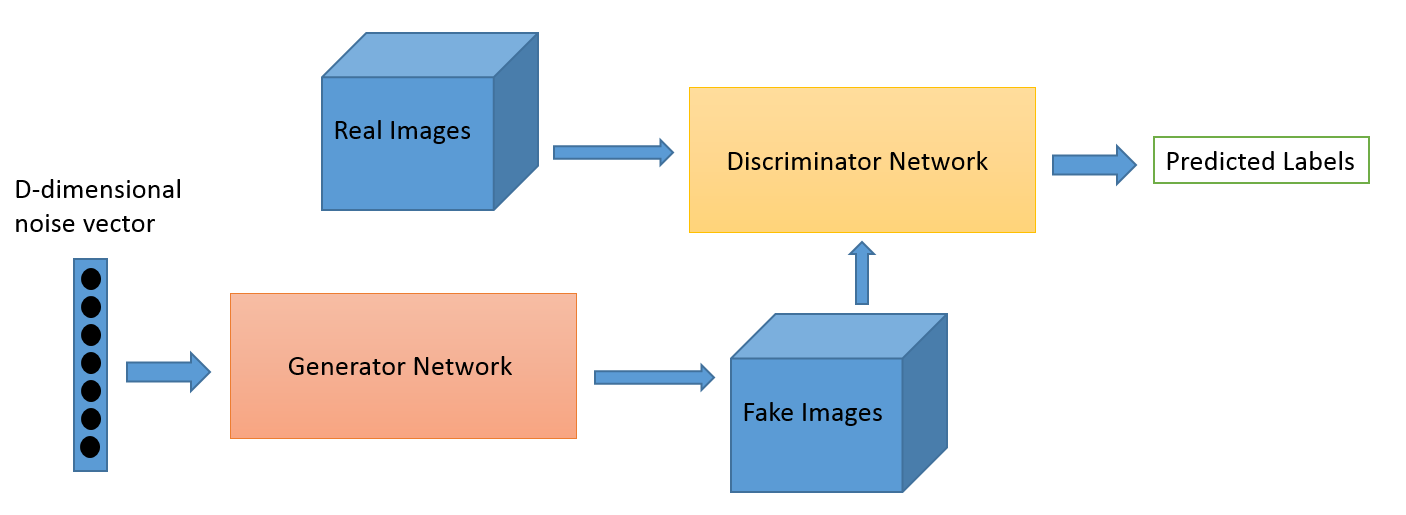
\includegraphics[width=12.5cm,height=5cm]{GAN.png}
\caption{\textsf{GAN} architecture}
\end{figure}
\vspace{3mm}

In the proposed adversarial nets framework, the generative model is pitted against an adversary: a discriminative model that learns to determine whether a sample is from the model distribution or the data distribution. The generative model can be thought of as analogous to a team of counterfeiters, trying to produce fake currency and use it without detection, while the discriminative model is analogous to the police, trying to detect the counterfeit currency. Competition in this game drives both teams to improve their methods until the counterfeits are indistiguishable from the genuine articles. 

A generator \texttt{G} and a discriminator \texttt{D} in \textsf{GAN} model play a zero-sum game. The training process is formulated as follows,
\begin{equation}
\arg \mathop{\min}_{G}\mathop{\max}_{D}V(D,G)=\mathbb{E}_{ \boldsymbol x\sim p_{data}(\boldsymbol x)} [\log D(\boldsymbol x)] + \mathbb{E}_{ \boldsymbol z\sim p_{ \boldsymbol z}(\boldsymbol z)} [\log {(1-D(G(\boldsymbol z)))}].
\end{equation}

The whole algorithm is listed as follows.

\begin{figure}[h]
\centering
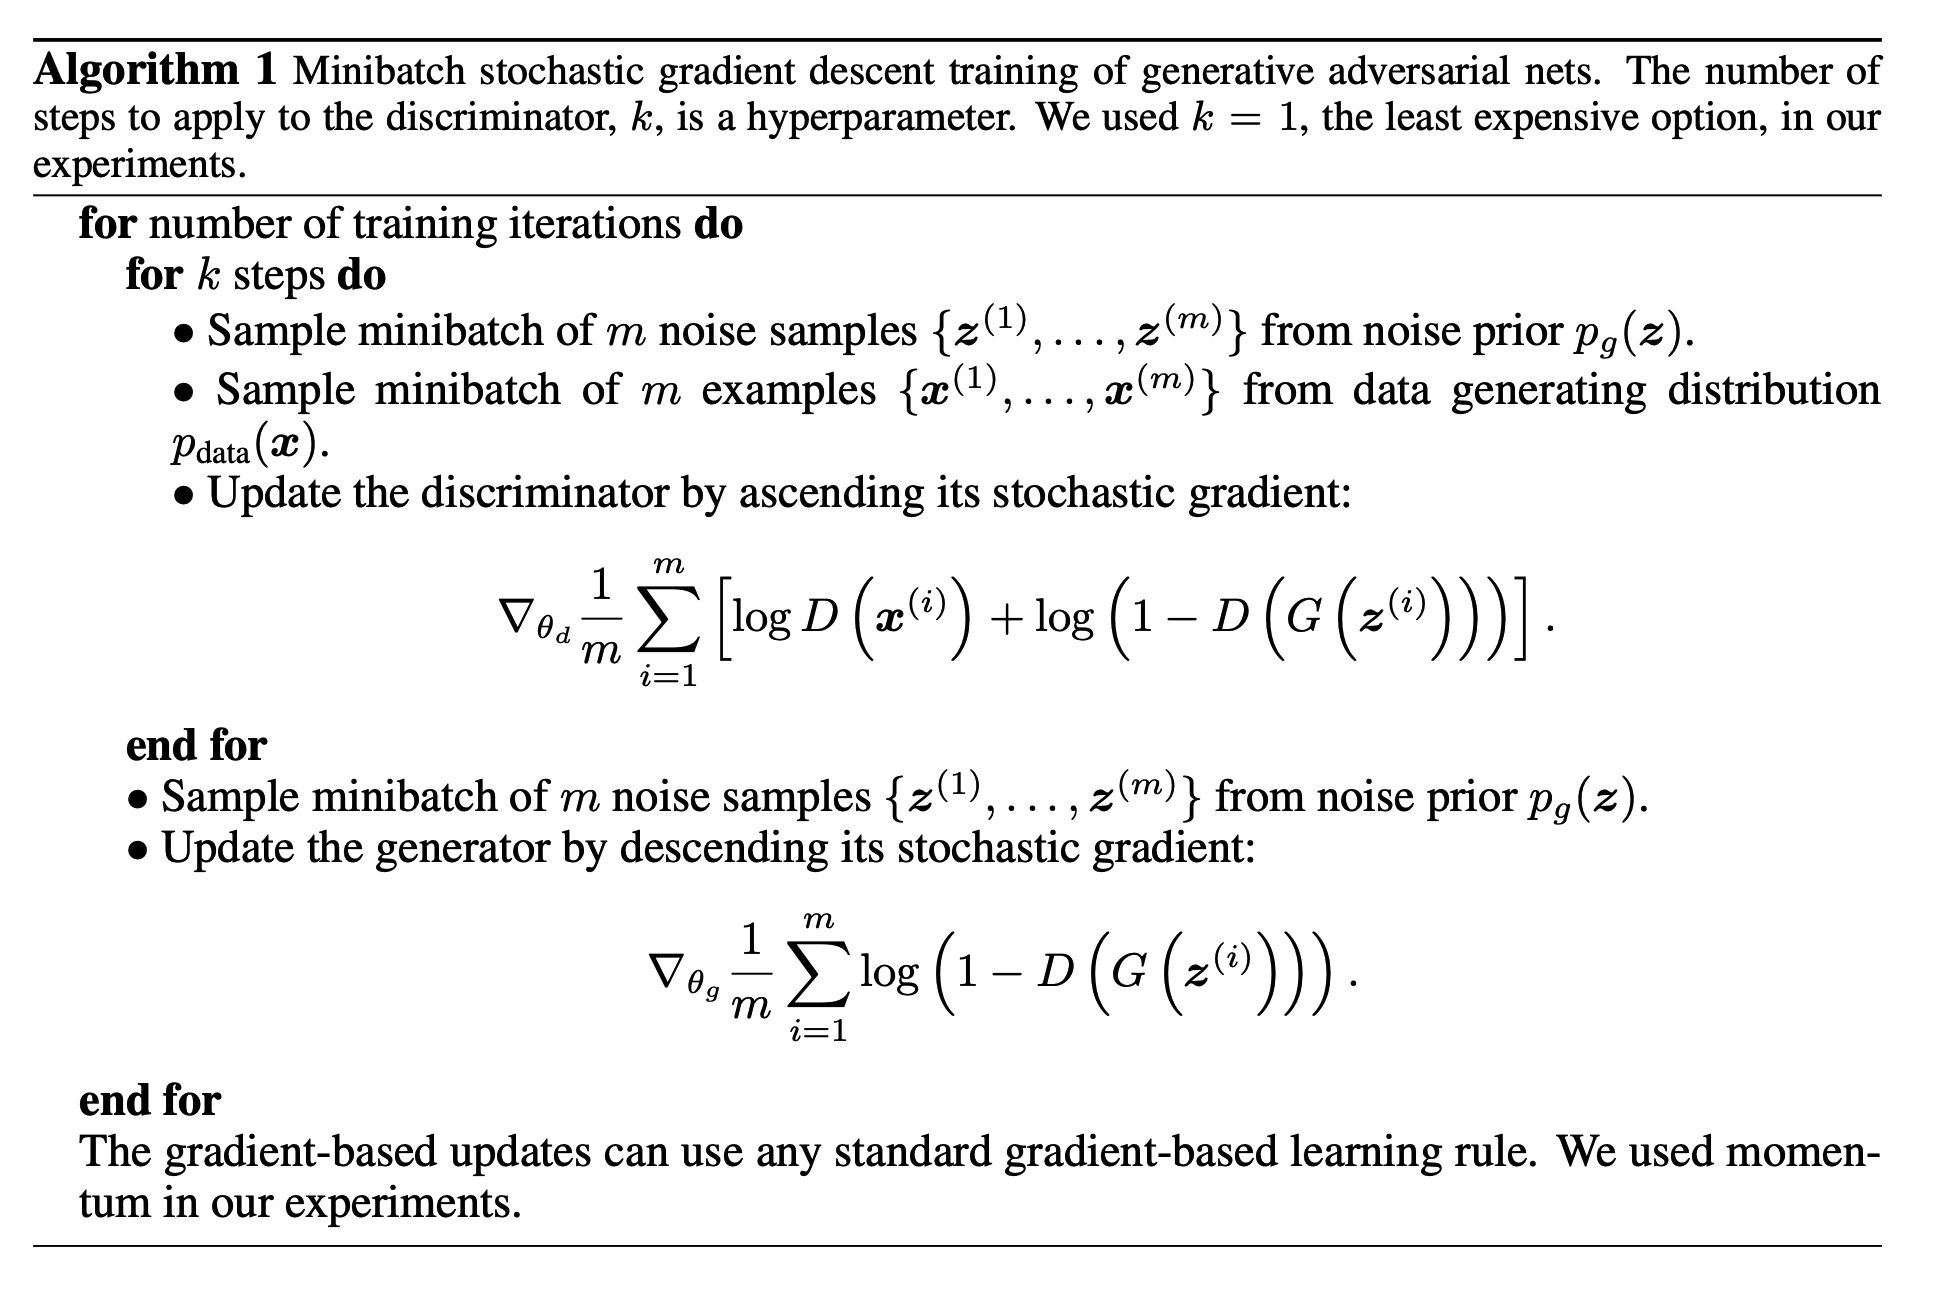
\includegraphics[width=14.8cm,height=9.75cm]{GANalg.png}
\end{figure}

Results in this paper demonstrates the viability of the adversarial modeling framework, suggesting that these research directions could prove useful.

\vspace{2mm}
\begin{center}
\large\textbf{Conditional Adversarial Networks}
\end{center}
\vspace{1mm}
\large{

Conditional generation is an enhancement of traditional models, including additional input conditional variables. The image-conditional models have tackled image prediction from a normal map, future frame prediction, product photo generation, and image generation from sparse annotations. Paper \href{https://arxiv.org/pdf/1611.07004.pdf}{\emph{Image-to-Image Translation with Conditional Adversarial Networks}} investigates conditional adversarial networks to image-to-image translation as a pioneer. The model in that paper can not only learn the mapping from input image to output image, but also learn a loss function to train this mapping problems. Widely-know as \textsf{Pix2Pix}, it's sufficient to generate good results.

\vspace{2mm}
\begin{figure}[H]
\centering
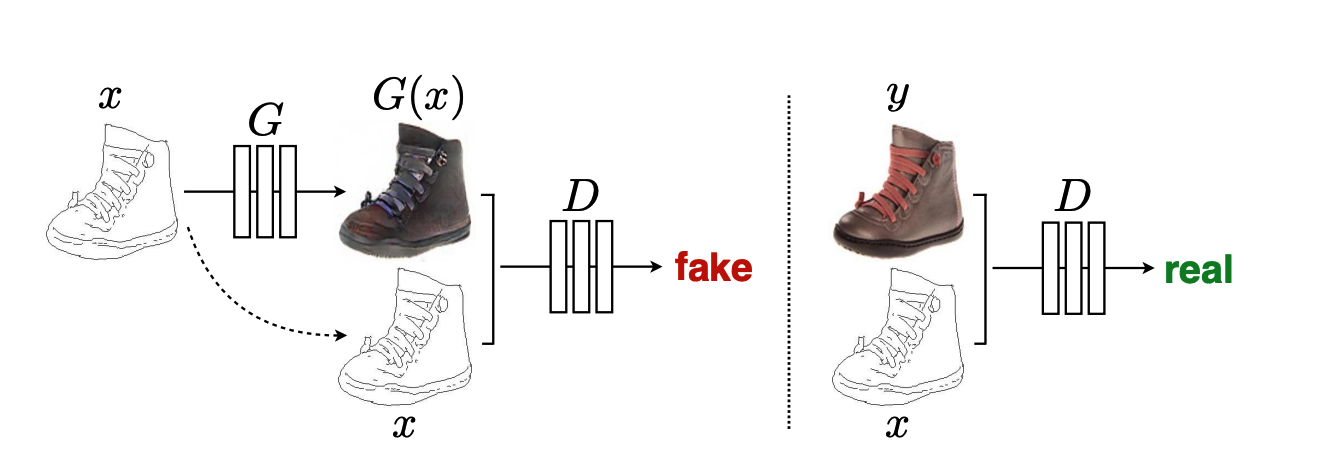
\includegraphics[width=12.5cm,height=4.58cm]{pix2pix.png}
\caption{\textsf{Pix2Pix} model for image-to-image transition}
\end{figure}
\vspace{2mm}

The principle behind is not sophisticated. The formula is re-defined as follows, 

\begin{equation}
\mathcal{L}_c GAN(G,D)=\mathbb{E}_{x,y} [\log D(x,y)] + \mathbb{E}_{x,z} [\log {(1-D(x,G(x,z))}].
\end{equation}

\begin{equation}
\mathcal{L}_{L1}(G)=\mathbb{E}_{x,y,z} [\|\log {(y-G(x,z))}\|_1].
\end{equation}

\begin{equation}
\arg \mathop{\min}_{G}\mathop{\max}_{D}\mathcal{L}_c GAN(G,D)+\lambda \mathcal{L}_{L1}(G).
\end{equation}
\vspace{2mm}

Results suggest that \textsf{Pix2Pix} are a promising approach for many image-to-image translation tasks, especially those involving highly structured graphical outputs. \textsf{Pix2Pix} learns a loss adapted to the task and data at hand, which makes them applicable in a wide variety of settings.

}


\vspace{5mm}
\begin{center}
\large\textbf{Cycle Consistency} \\
\end{center}

\large{
The idea of using transitivity as a way to regularize structured data has a long history. In visual tracking, enforcing simple forward-backward consistency has been a standard trick for decades. In the language domain, verifying and improving translations via “\emph{back translation and reconciliation}” is a technique used by human translators, as well as by machines. Paper \href{http://openaccess.thecvf.com/content_cvpr_2016/papers/Zhou_Learning_Dense_Correspondence_CVPR_2016_paper.pdf}{\emph{Learning Dense Correspondence via 3D-guided Cycle Consistency}} establishes dense visual correspondence across different object instances.}

\vspace{3mm}
\begin{figure}[H]
\centering
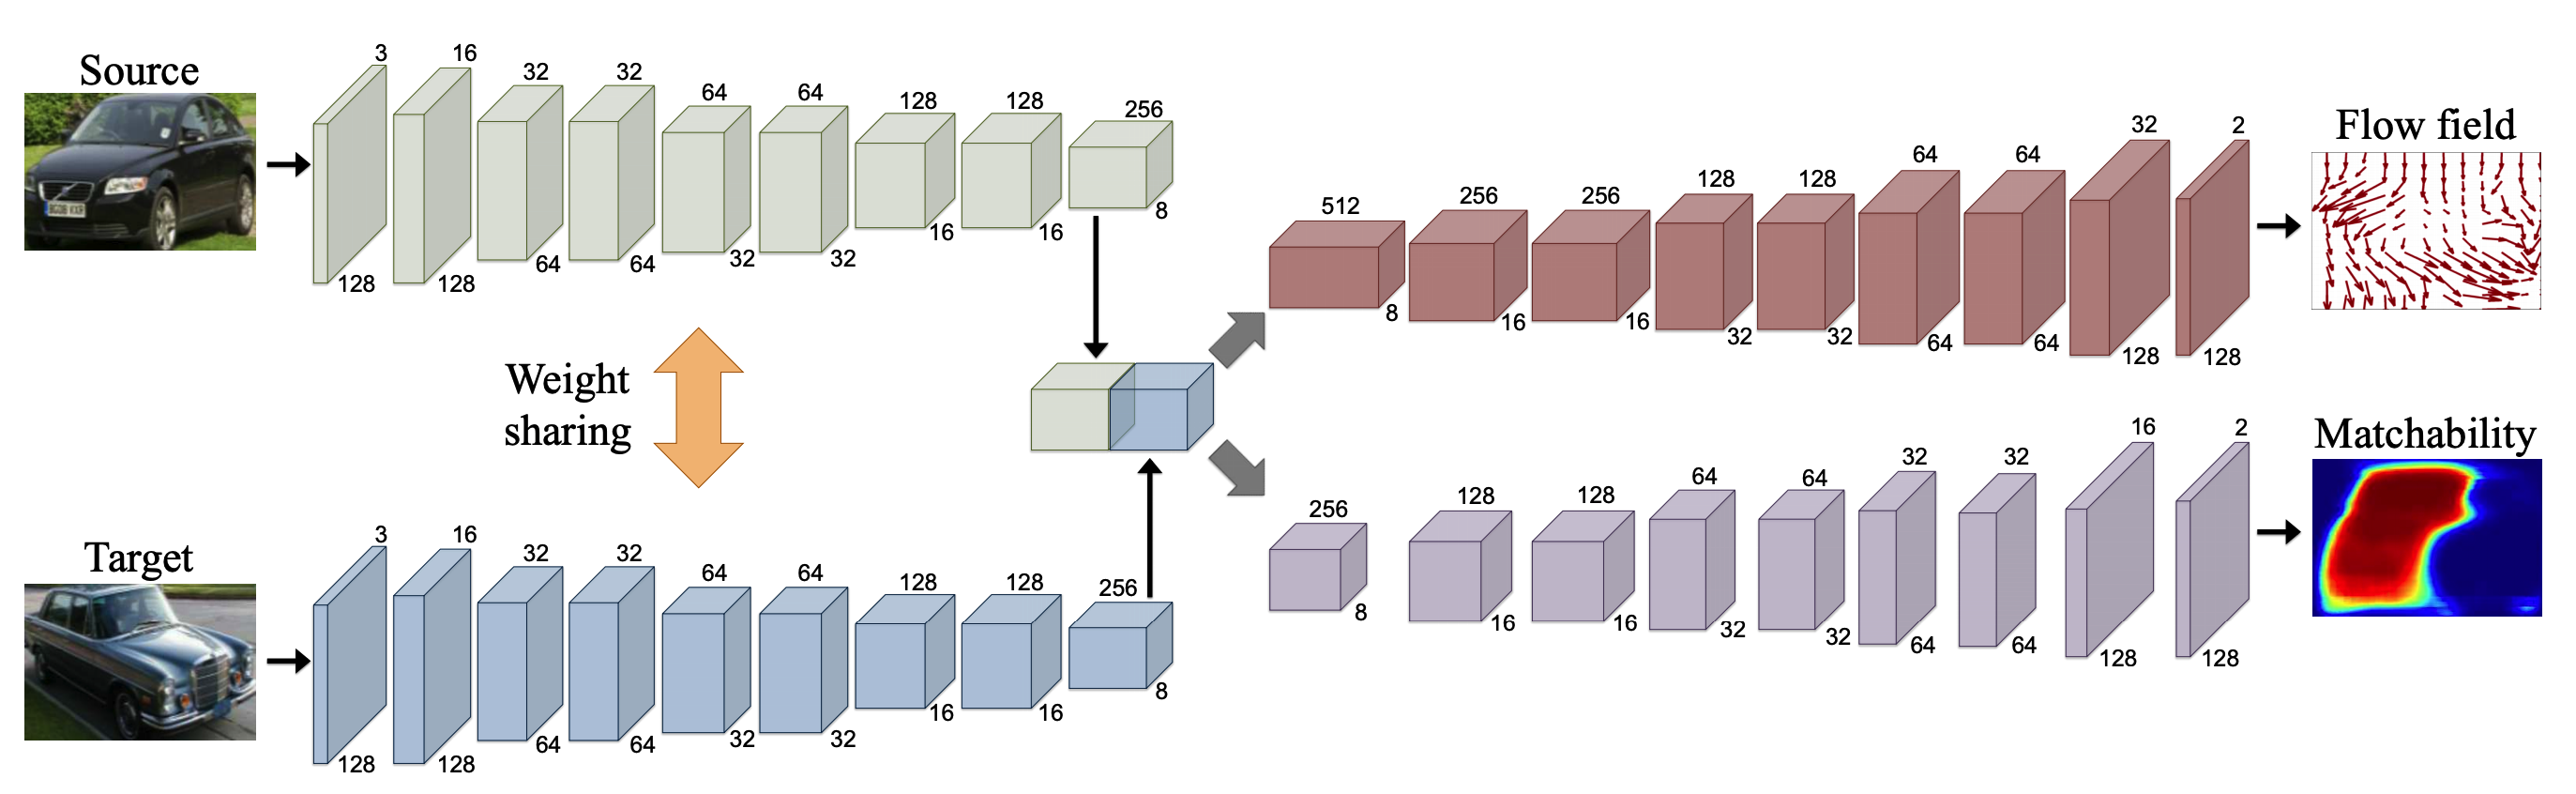
\includegraphics[width=12.5cm,height=4.1cm]{cycleconsistence.png}
\caption{Learning Dense Correspondence via 3D-guided Cycle Consistency}
\end{figure}
\vspace{2mm}

\clearpage

%%
\vspace{5mm}
\begin{center}
\LARGE\textbf{II. Model} \\
\end{center}
\vspace{2mm}

\vspace{2mm}
\begin{center}
\large\textbf{Architecture} \\
\end{center}


\large{
Aim to capture special characteristics of one image collection and figuring out how these characteristics could be translated into the other image collection, all in the absence of any paired training examples, the paper tries to exploit an algorithm that can learn to translate between domains without paired input-output examples. The framework is shown as \textbf{Fig. \ref{cyclegan}}.

\vspace{3mm}
\begin{figure}[H]
\centering
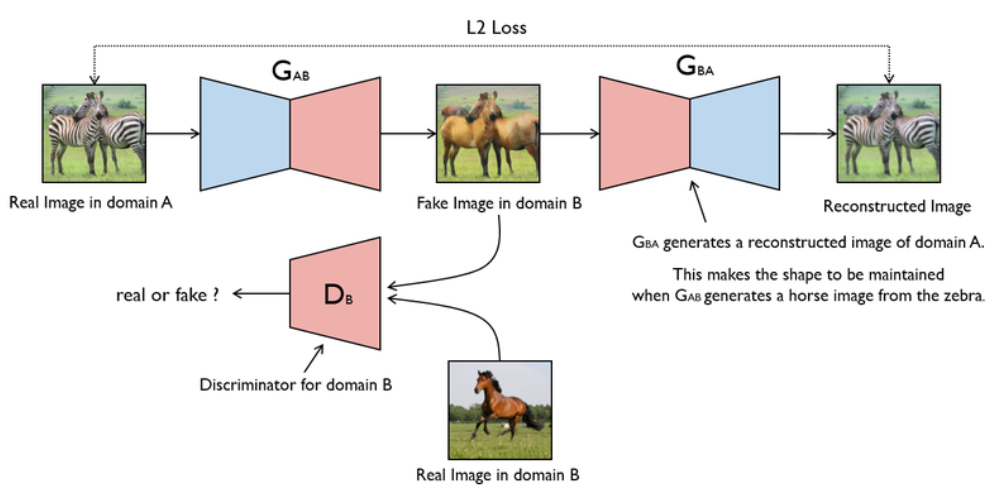
\includegraphics[width=12.5cm,height=6.66cm]{cyclegan.png}
\caption{\textsf{Cycle-GAN architecture}}
\label{cyclegan}
\end{figure}
}

%%%%%
\vspace{5mm}
\begin{center}
\large\textbf{Algorithm} \\
\end{center}

\large{Our goal is to learn mapping functions between two domains $X$ and $Y$. We denote the data distribution as $\boldsymbol x \sim p_{data}(\boldsymbol x)$ and $\boldsymbol y \sim p_{data}(\boldsymbol y)$. \textsf{Cycle-GAN} model includes 2 mappings: $G:X \rightarrow Y$ and $F: Y\rightarrow X$. \textsf{Cycle-GAN} introduces 2 adversarial discriminators $D_X$ and $D_Y$, where $D_X$ aims to distinguish between images $\{x\}$ and translated images $\{ F(y) \}$; in the same way, $D_Y$ aims to discriminate between $\{y\}$ and $\{G(x)\}$. Our objective contains two types of terms: 

\begin{itemize}
    \item \textbf{Adversarial losses:} matches the distribution of generated images to the data distribution in the target domain.
    \item \textbf{Cycle Consistency losses:} serves to prevent the learned
mappings G and F from contradicting each other.
\end{itemize}

\begin{align}
    \mathcal{L}_{GAN}(G,D_y,X,Y)=&\mathbb{E}_{ \boldsymbol y\sim p_{data}(\boldsymbol y)} [\log D_Y(\boldsymbol y)] \notag \\
    &+ \mathbb{E}_{ \boldsymbol x\sim p_{data}(\boldsymbol x)} [\log {(1-D_Y(G(\boldsymbol x)))}].
\end{align}
\begin{align}
    \mathcal{L}_{cyc}(G,F)=&\mathbb{E}_{ \boldsymbol x\sim p_{data}(\boldsymbol x)} [\|F(G(\boldsymbol x))-\boldsymbol x\|_1] \notag \\ 
    &+ \mathbb{E}_{ \boldsymbol y\sim p_{data}(\boldsymbol y)} [\|G(F(\boldsymbol y))-\boldsymbol y\|_1].
\end{align}
\begin{align}
    \arg \mathop{\min}_{G,F}\mathop{\max}_{D_{X},D_{Y}}\mathcal{L}(G,F,D_X,D_Y)=&\mathcal{L}_{GAN}(G,D_y,X,Y) \notag\\
    &+\mathcal{L}_{GAN}(G,D_X,Y,X)\notag\\
    &+\mathcal{L}_{cyc}(G,F).
\end{align}

}

\vspace{5mm}
\begin{center}
\LARGE\textbf{III. Experiments} \\
\end{center}

\vspace{2mm}
\begin{center}
\large\textbf{Metrics} \\
\end{center}

\large{We keep an image buffer that stores the 50 previously created images. For all the experiments, we set $\lambda$ = 10. We use the Adam solver with SGD. All networks were trained from scratch with a learning rate of 0.0002. We keep the same learning rate for the first 100 epochs and linearly decay the rate to zero over the next 100 epochs.}

%%%%%
\vspace{2mm}
\begin{center}
\large\textbf{Implementation} \\
\end{center}

\large{You can view our whole implementation in \textbf{Appendix.} B.

The network contains two stride-2 convolutions, several residual blocks, and two fractionally strided convolutions with stride .5. We use 6 blocks for 128 * 128 images and 9 blocks for 256 * 256 and higher resolution training images. Similar to Johnson et al., we use instance normalization. For the discriminator networks we use 70 * 70 \textsf{Patch-GANs}, which aim to classify whether 70 * 70 overlapping image patches are real or fake.}

%%%%%
\vspace{2mm}
\begin{center}
\large\textbf{Results} \\
\end{center}

\large{

\vspace{3mm}
\begin{figure}[h]
\centering
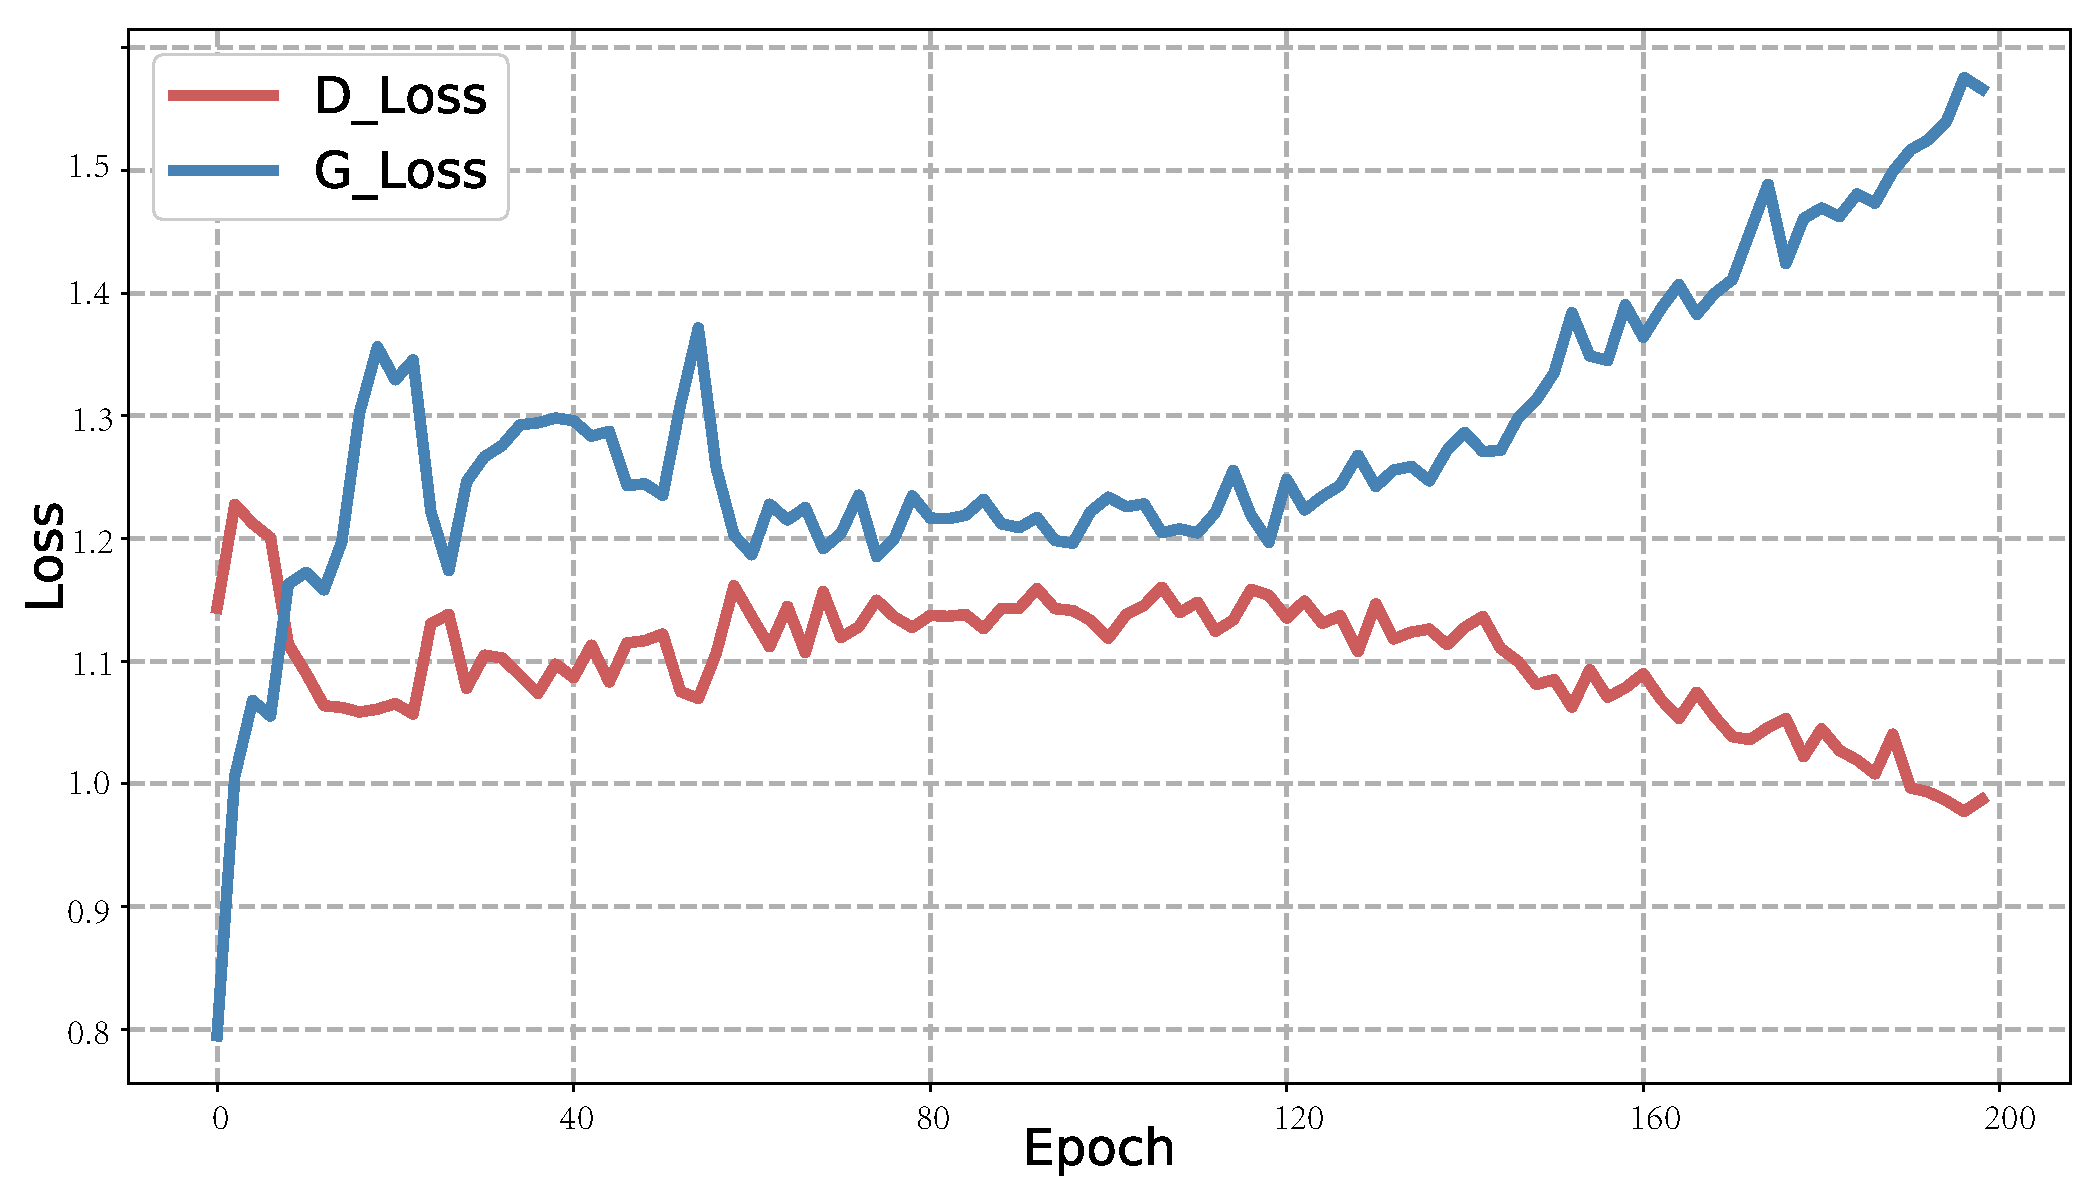
\includegraphics[width=13.5cm,height=8.2cm]{losses.pdf}
\caption{Results with training (Monet painting versus photograph)}
\label{losses}
\end{figure}
\vspace{2mm}

\textbf{Fig. \ref{losses} }shows the loss of generator and discriminator in 200 epoch respectively. Note that the growth trend of the two curves is opposite, indicating the antagonism between them.


\vspace{3mm}
\begin{figure}[h]
\centering
\includegraphics[width=15cm,height=15cm]{cycleGAN.pdf}
\caption{Results with training in various datasets.}
\label{moreresults}
\end{figure}
\vspace{2mm}

\large\textbf{Fig. \ref{moreresults}} shows the process of the experiment from the early stage to final stage in several datasets, (i.e. \texttt{Vango2Photo}, \texttt{Monet2Photo}, and \texttt{Summer2Winter}). The early stage usually refers to the first 5 epoch, while the final stage refers to the last 5 epoch. From this illustration, we can clearly see that the outcomes become more clearly, and differences of results exist in these transitions. Results become more authentic with the training, changing from random noise to fakes which are difficult to identify. 
} 

%%%%%
\vspace{2mm}
\begin{center}
\large\textbf{Evaluation} \\
\end{center}

\large{To show the advancement of applying \textsf{Cycle-GAN} to image style transfer, we adopt the following approaches to evaluate this method. Note that we do not implement all of the neural networks on different evaluation platform, so the results may partially come from the original paper. 

First, we compare our results with some baseline algorithms, (\textit{i.e.}, \textsf{Go-GAN}, \textsf{Bi-GAN}, \textsf{Feature Loss} + \textsf{GAN}, and \textsf{Pixel Loss} + \textsf{GAN}). Running “real vs fake” perceptual studies on Amazon Mechanical Turk (\textbf{AMT}), we assess the realism of our outputs. \textbf{Table. 1}.} Observing the results of these methods, we can find that \textsf{Cycle-GAN} has higher accuracy towards others, both from Map $\to$ Photo and from Photo $\to$ Map. 

\vspace{2mm}
\renewcommand{\baselinestretch}{1.3}
\begin{table}
\begin{center}
\begin{tabular}{ccc} 
\hline
\textbf{Loss}& \textbf{Map $\to$ Photo} & \textbf{Photo $\to$ Map}\\
\hline
\textsf{Go-GAN}&0.6\%$\pm$0.5\%&0.9\%$\pm$0.5\%\\
\textsf{Bi-GAN}&2.1\%$\pm$1.0\%&1.9\%$\pm$0.9\%\\
\textsf{Pixel Loss}+\textsf{GAN}&0.7\%$\pm$0.5\% &2.6\%$\pm$1.1\%\\
\textsf{Feature Loss}+\textsf{GAN}&1.2\%$\pm$0.6\%&0.3\%$\pm$0.2\%\\
\textsf{Cycle-GAN}& \textbf{26.8}\%$\pm$\textbf{2.8}\%&\textbf{23.2}\%$\pm$\textbf{3.4}\%\\
\hline
\end{tabular}
\end{center}
\caption{AMT “real vs fake” test on maps $\to$ aerial photos.}
\end{table}
\renewcommand{\baselinestretch}{1.0}
To prove the realism of the generated images of \textsf{Cycle-GAN}, we also use FCN metric. FCN metric evaluates how interpretable the generated photos are according to an off-the-shelf semantic segmentation algorithm (the fully-convolutional network, FCN). In this reimplementation, FCN is used to predict a label map for a generated photo, which can then be compared against the input ground truth labels. We conduct our experiments on the \texttt{Cityscapes} dataset. \textbf{Table. 2}. assesses the performance of the labels $\to$ photo task on the \texttt{Cityscapes}. Similarly, \textbf{Table. 3} evaluates the opposite mapping. In both cases, \textsf{Cycle-GAN} outperforms the baseline methods, which proves the advancement of \textsf{Cycle-GAN} on image style transfer.
\renewcommand{\baselinestretch}{1.5}
\begin{table} 
\begin{center}
\begin{tabular}{cccc} 
\hline
\textbf{Loss}& \textbf{Per-pixel acc.} & \textbf{Per-class acc.}&\textbf{Class IOU}\\
\hline
\textsf{Go-GAN}&0.40&0.10&0.06\\
\textsf{Bi-GAN}&0.19&0.06&0.02\\
\textsf{Pixel Loss}+\textsf{GAN}&0.20&0.10&0.04\\
\textsf{Feature Loss}+\textsf{GAN}&0.06&0.04&0.01\\
\textsf{Cycle-GAN}&\textbf{0.52}&\textbf{0.17}&\textbf{0.11}\\
\hline
\textsf{pix2pix}&0.71&0.25&0.18\\
\end{tabular}
\end{center}
\caption{FCN-scores of labels $\to$ photos for different methods.}
\end{table}

\begin{table} 
\begin{center}
\begin{tabular}{cccc} 
\hline
\textbf{Loss}& \textbf{Per-pixel acc.} & \textbf{Per-class acc.} &\textbf{Class IOU}\\
\hline
\textsf{Go-GAN}&0.45&0.11&0.08\\
\textsf{Bi-GAN}&0.41&0.13&0.07\\
\textsf{Pixel Loss}+\textsf{GAN}&0.47&0.11&0.07\\
\textsf{Feature Loss}+\textsf{GAN}&0.50&0.10&0.06\\
\textsf{Cycle-GAN}&\textbf{0.58}&\textbf{0.22}&\textbf{0.16}\\
\hline
\textsf{pix2pix}&0.85&0.40&0.32\\
\end{tabular}
\end{center}
\caption{Classification performance of photos $\to$ labels for different methods.}
\end{table}
\renewcommand{\baselinestretch}{1.0}
Limited by energy and time, we have not achieved all the results of this paper. You are able to obtain a comprehensive results on \href{https://junyanz.github.io/CycleGAN/}{this website}. Besides, Zhu et. al. do many extensive evaluation experiments, like comparing different loss methods, doing ablation studies, and making some paired dataset comparison. View the original article to get more results and evaluations!

%%
\vspace{10mm}
\begin{center}
\LARGE\textbf{IV. Conclusion} \\
\end{center}
\vspace{2mm}

In this report, we implement the code of \href{https://arxiv.org/pdf/1703.10593.pdf}{\emph{``Unpaired Image-to-Image Translation using Cycle-Consistent Adversarial Networks''}}. \textsf{Cycle-GAN} stands on the shoulder of some splendid previous work show great performance when applied to style transaction. We modify the original code of the paper and train the model for \textbf{about a month}. We also evaluate this method by comparing with some other popular approaches on \texttt{Cityscape} dataset and discover that \textsf{Cycle-GAN} outperform the others both from labels to photos and from photos to labels. We born the midnight oil and eventually get the trained models and results. Although this experiment was concluded temporarily, the research on \textsf{Cycle-GAN} do not stop -- many enhanced model come one after another just in the following two years (2018-2019). This experiment of reimplementing give us a deeper understanding of General Adversarial Network and encourage us to devote to deep learning the whole life.

%%
\vspace{1cm}
\begin{center}
\LARGE\textbf{V. Acknowledgement} \\
\end{center}
\vspace{.5mm}

\begin{itemize} \item{First and foremost, I would like to show my deepest gratitude to my teacher, professor \textbf{Roy Wang}, who has provided us with valuable theoretical guidance of deep learning. Without his enlightening instruction, impressive kindness and patience, I could never have completed our projects. His keen and vigorous academic observation enlightens me in this thesis and my future study.}
\item{My sincere appreciation also goes to our \textbf{teacher assistants}. We got along in harmony. They also gave me valuable advice. All of these make this experience meaningful.}
\end{itemize}

\clearpage
%%
\vspace{5mm}
\begin{center}
\LARGE\textbf{VI. Appendices} \\
\end{center}
\vspace{1mm}
\begin{center}
\large\textbf{A. Brief History of NST} \\
\end{center}
The power of Convolutional Neural Networks (\textbf{CNNs}) is gradually discovered in creating artistic imagery by separating and recombining image content and style. Since then, NST has become a trending topic both in academic literature and industrial applications.

Inspired by the power of Convolutional Neural Networks (CNNs), Gatys et al. first studied how to use a CNN to reproduce famous painting styles on natural images, which opens the doors of deep-learning applied approaches to solving the style transfer problem. They modeled the content of a photo as the feature responses from a pre-trained CNN, and further model the style of an artwork as the summary feature statistics. This pioneer has given rise to a wave of work to transfer the neural network style. Branches of image style transfer emerge in the recent years can be roughly classified as shown in \textbf{Fig. \ref{review}}.

\vspace{4mm}
\begin{figure}[H]
\centering
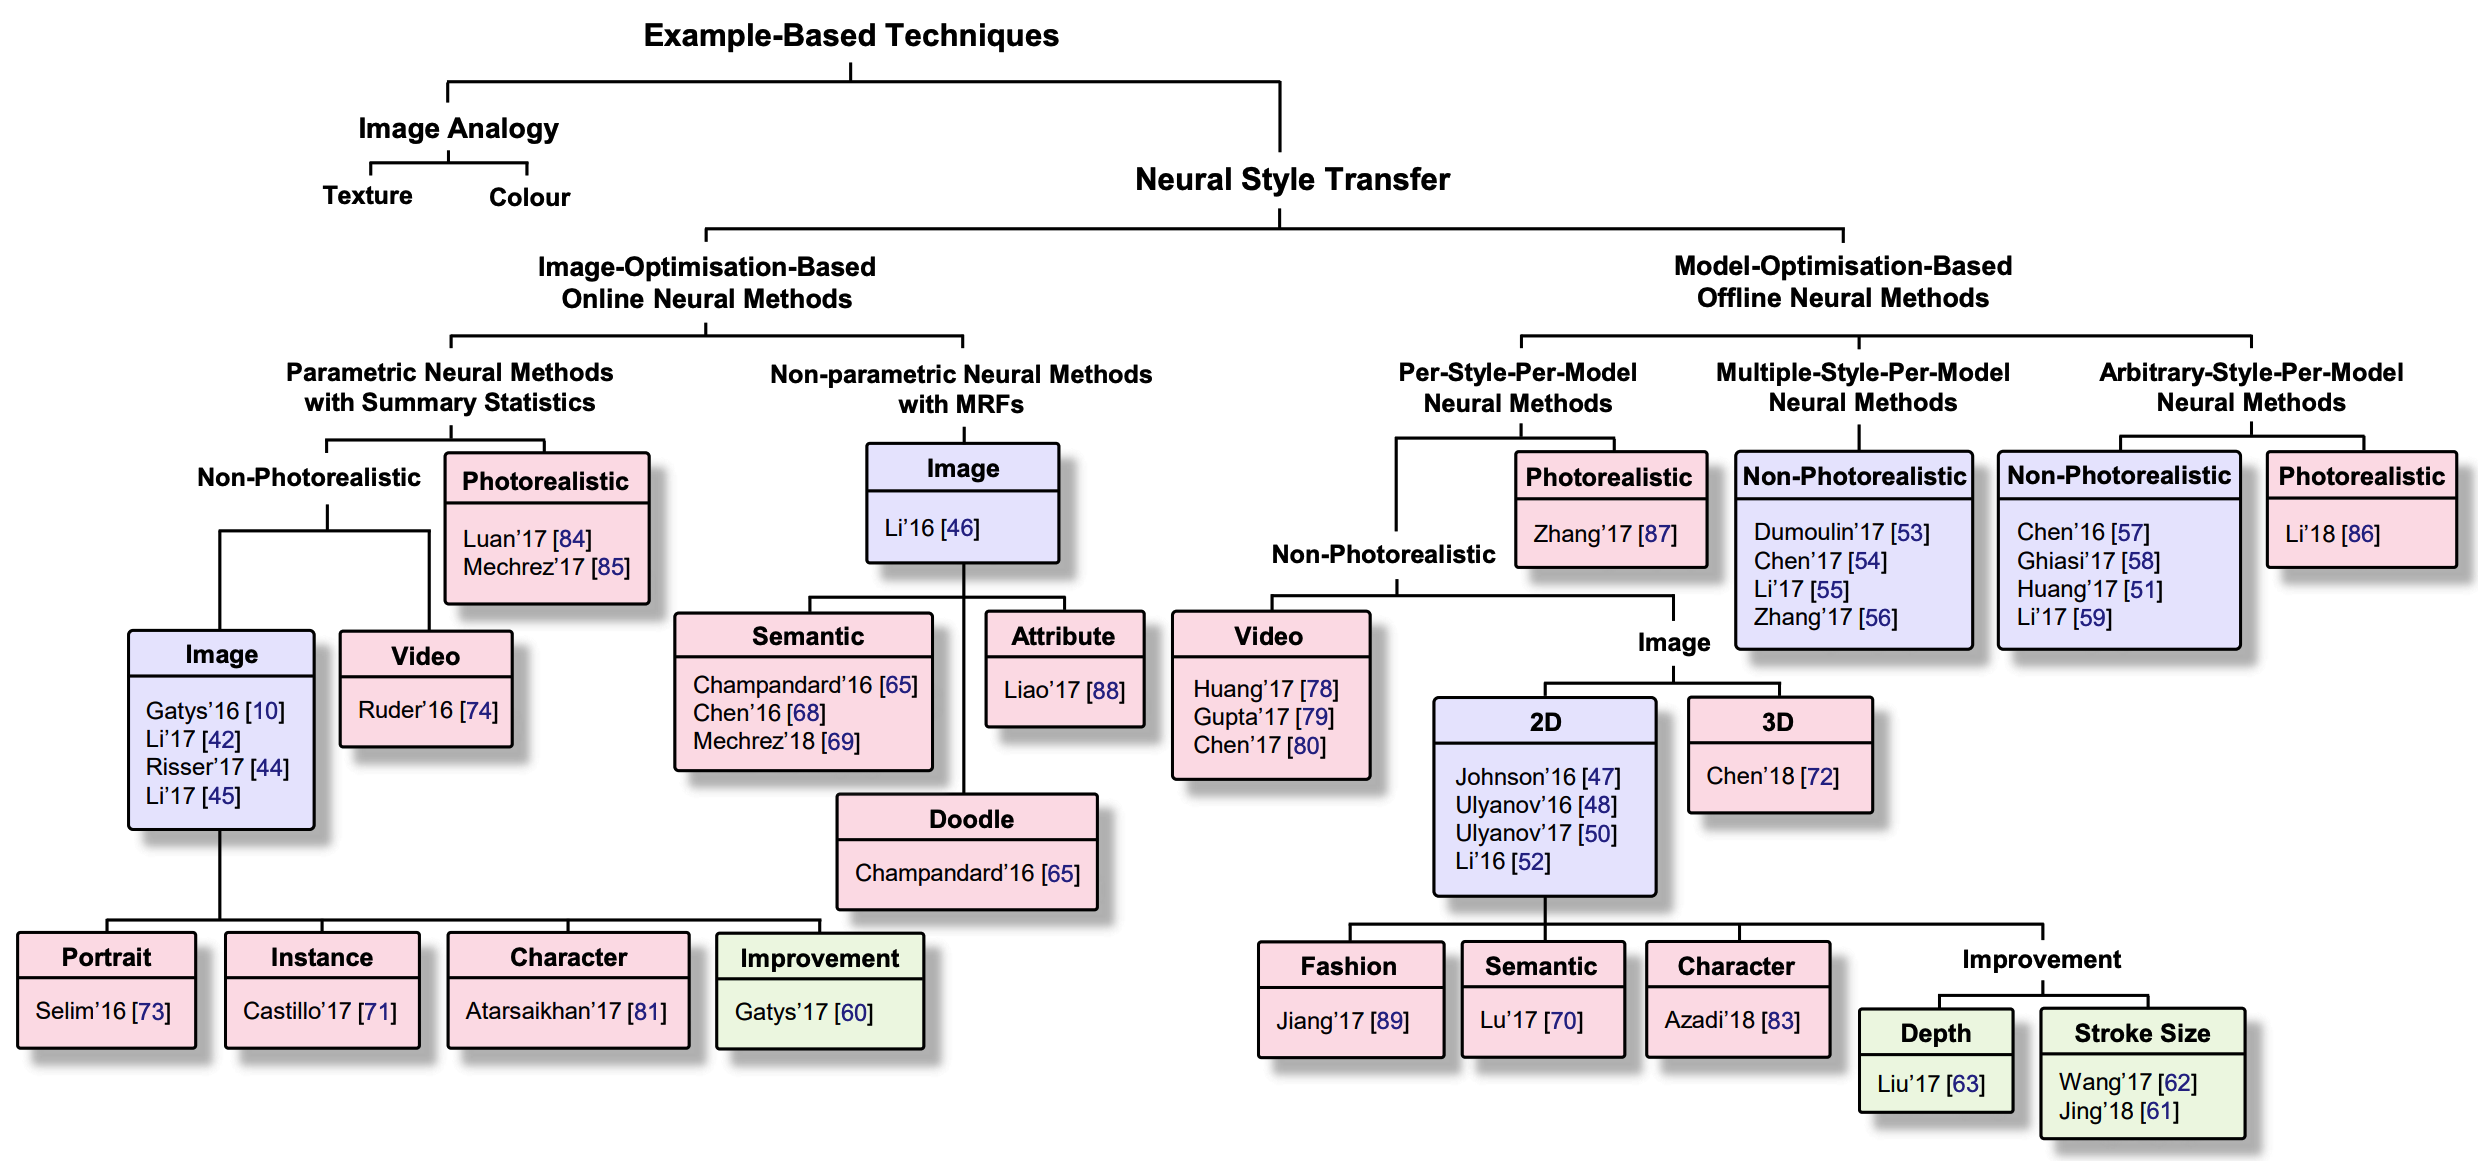
\includegraphics[width=15cm]{review.png}
\caption{Branches of image style transfer studies (\textit{by Jing et. al. in \href{https://arxiv.org/pdf/1705.04058.pdf}{Neural Style Transfer: A Review}}).}
\label{review}
\end{figure}

Despite the great progress in recent years, the area of NST is far from mature. Currently, the first stage of NST is to refine and optimise recent NST algorithms, aiming to perfectly imitate varieties of styles. This stage involves two technical directions. The first one is to reduce failure cases and improve stylised quality on a wider variety of style and content images; and the other technical direction lies in deriving more extensions from general NST algorithms. After moving beyond the first stage, a further trend of NST is to not just imitate human-created art with NST techniques, but rather to create a new form of AI-created art under the guidance of underlying aesthetic principles.


\clearpage
\begin{center}
\large\textbf{B. Code Implementation} \\
\end{center}


\vspace{2mm}
\large\noindent{
Code implementation is a fine-tuning, referring \href{https://github.com/hindupuravinash/the-gan-zoo}{\underline{\textsf{GAN} Zoo}} and \href{https://github.com/junyanz/pytorch-CycleGAN-and-pix2pix}{\underline{Paper Implementation}}.
}
\vspace{.5cm}

\noindent \LARGE \textsc{1) datasets.py} \small

\noindent \HRule

\lstinputlisting[language=python]{./datasets.py}

\noindent \HRule

\vspace{1cm}

\noindent \LARGE \textsc{2) utils.py} \small

\noindent \HRule

\lstinputlisting[language=python]{./utils.py}

\noindent \HRule

\vspace{1cm}

\noindent \LARGE \textsc{3) models.py} \small

\noindent \HRule

\lstinputlisting[language=python]{./models.py}

\noindent \HRule

\vspace{1cm}

\noindent \LARGE \textsc{4) cycleGAN.py} \small

\noindent \HRule

\lstinputlisting[language=python]{./cycleGAN.py} 

\noindent \HRule

\clearpage
\renewcommand{\baselinestretch}{1.3}
\begin{center}
\large\textbf{C. More Resource} \\
\end{center}
\vspace{2mm}
\large{During the experiment, we endured a tough period of training the model for about one month, we realize the importance of offloading the repeated training. Considering that the pursuit of fast and convenient training, we upload our pre-trained model on Baidu Cloud Service. 

Click \href{https://pan.baidu.com/s/1qb6ye6ZszvrdTRdHItjuqg}{\underline{\textit{this link}}} to down the pre-trained models and demo images!

Besides, we upload the source code on GitHub, \href{https://github.com/LovelyBuggies/Jupyter_DeepLearning_Homework/tree/master/Cycle-GAN}{\underline{\textit{click here}}} to see the code online!
}
\end{document}
